\chapter{Fundamentos de las redes neuronales} \label{Capitulo_2}
\begin{itemize}
	\item Supervisado y no supervisado
	\item one-hot encoder
	\item validacion cruzada
	\item dropout, l2
	\item optiizadores
	\item arquitectuas
	\item metricas
\end{itemize}
en la pagina 458 de hands aparece la arquitectura mía


\section{Revisión teórica} \label{Subsec: 3_1}
Puedo introducir los tipos de funciones de activavion. Esta bien explicado en el TFG wuolah o en el articulo de KDD cup 199 de DNN network intrusion.
Puedo añadir overfitting y underfitting.
lo que es aprendizaje supervisado y no supervisao
Partes de una neurona y como trabaja(bias, pesos...)


\section{Arquitecturas relevantes} \label{Subsec: 3_2}
Mini tabla resumen en Deep Cybersecurity: A Comprehensive Overview from Neural Network and Deep Learning Perspective y miniresumen de todos los tipos en review Deep Cybersecurity: A Comprehensive Overview from Neural Networkand Deep Learning Perspective y review

\subsection{Autoencoder}

Los autoencoders son una clase de redes neuronales artificiales utilizadas en aprendizaje no supervisado para aprender representaciones eficientes de los datos. Su funcionamiento consiste en codificar la entrada en una representación comprimida y significativa, y luego decodificarla de manera que la reconstrucción sea lo más similar posible a la entrada original \citep{lopes2022effective}. La arquitectura básica de un autoencoder consta de tres partes: el encoder, el cuello de bottela y el decoder (Figura \ref{fig:AE_architecture}). 

\begin{figure}[h]
    \centering
    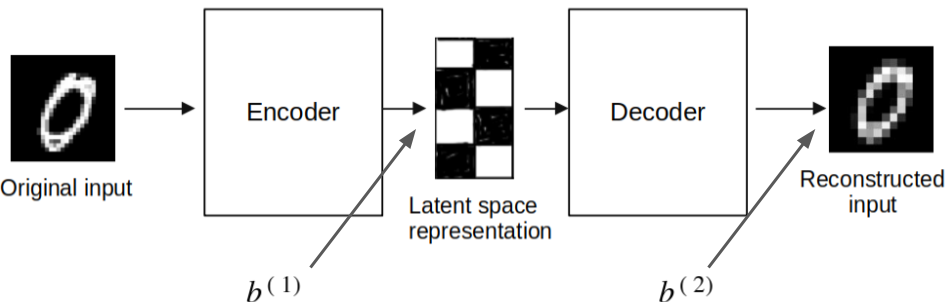
\includegraphics[width=0.6\textwidth]{img/AE0.png}
    \caption{Arquitectura de un autoencoder. Fuente:\citep{autoencoderImage}.}
    \label{fig:AE_architecture}
\end{figure}

El encoder mapea los datos de entrada a una representación oculta de menor dimensión utilizando funciones principalmente no lineales, mientras que el decoder reconstruye los datos de entrada a partir de esta representación oculta. Durante el entrenamiento, los parámetros del autoencoder se optimizan para minimizar la diferencia entre la entrada y la salida reconstruida, utilizando una función de pérdida que mide esta discrepancia, como por ejemplo la pérdida de entropía cruzada.


Las ecuaciones para obtener la salida de un autoencoder serían:
\[
\left\{
\begin{aligned}
z^{(1)} &= W^{(1)} \cdot x + b^{(1)} \\
a^{(2)} &= f(z^{(1)})  \\
z^{(2)} &= W^{(2)} \cdot a^{(2)} + b^{(2)}  \\
y &= z^{(2)} 
\end{aligned}
\right.
\]

donde  $x$ es el input, \( b^{(1)} \) y  \( b^{(2)} \) son los sesgos,  \( W^{(1)} \) y  \( W^{(2)} \) son los pesos, \( z^{(1)} \) es la salida lineal de la primera capa, \( a^{(2)} \) es la activación de la segunda capa, \( z^{(2)} \) es la salida lineal de la segunda capa e \( y \) es la salida final del modelo \citep{martinez2017analisis}.


Los autoencoders se utilizan en una amplia variedad de aplicaciones, incluida la reducción de dimensionalidad, la extracción de características, la eliminación de ruido en los datos de entrada y la detección de anomalías. Su versatilidad y capacidad para aprender representaciones útiles de los datos los hacen herramientas poderosas.


Las principales capas que se utilizan en esta red neuronal son las capas densas y las de aplanamiento, aunque también se pueden utilizar capas convolucionales y de pooling para autocodificadores convolucionales\footnote{Autocodificador para imágenes de gran tamaño} o LSTM en el caso de autocodificadores recurrentes\footnote{Autocodificador específico para series temporales o secuencias.}\citep{geron2022hands}. 






\subsection{Deep Belief Networks}
\subsubsection{Red Neuronal Profunda}
\subsection{Red Neuronal Convolucional}


Las redes neuronales convolucionales son una de las métodos de machine learning más importantes y utilizados en el campo de la ciberseguridad. Estas redes neuronales están diseñadas para procesar entradas almacenadas en matrices, como las imágenes.  Estas redes son una parte de las redes neuronales profundas que procesa y analiza entradas de imágenes visuales, y están compuestas por neuronas con pesos y sesgos que aprenden a lo largo de su entrenamiento \citep{podder2021artificial}. La arquitectura de una CNN (Figura \ref{fig:cnn_architecture}) consta de tres tipos de capas: capas de convolución, capas de pooling y la capa de clasificación. 
 

\begin{figure}[h]
    \centering
    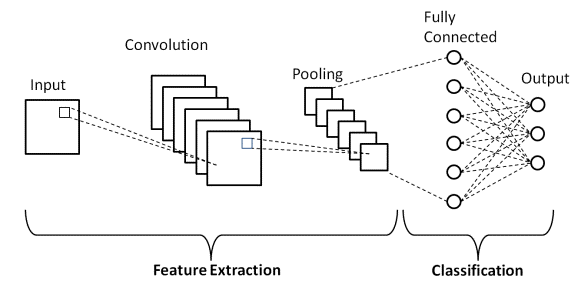
\includegraphics[width=0.6\textwidth]{img/convlayers.png}
    \caption{Arquitectura de una CNN con capas de convolución, pooling y clasificación. Fuente:\citep{phung2018deep}.}
    \label{fig:cnn_architecture}
\end{figure}

\subsubsection*{Capas convolucionales}

La capa convolucional es la capa más importante de una \acrshort{cnn}. En ella se extraen las características más significativas de la imagen de entrada, como los bordes, el color o la forma. Para ello se aplica una convolución a la imagen con un filtro. Esta operación matemática se representa como \( \int (x \star w)(t) \) donde $x$ representa la entrada y $w$ el núcleo de convolución \citep{pajares2021aprendizaje}.



En una CNN, la entrada de la convolución es una matriz multidimensional mientras que $w$ es una matriz de parámetros, llamada núcleo o filtro, que se ajusta durante el aprendizaje.
Cada píxel de la capa de convolución tiene una neurona, que se conecta con la capa anterior aplicando la convolución con las neuronas de su campo receptivo\footnote{Región de entrada que contribuye a la salida generada por el filtro} \cite{geron2022hands}. Esta convolución se realiza con un solapamiento total del filtro, lo que resulta en una imagen de menor dimensión (Figura \ref{fig:convolucion}). Si se desea mantener la misma dimensión, se puede aplicar zero-padding, que consiste en rellenar con ceros la matriz para obtener las dimensiones deseadas (Figura \ref{fig:convolucionPadding}). En la figura \ref{fig:convolu2} se muestran sendos campos receptivos de la imagen \( I \) que contribuyen a las salidas \( P \) y \( Q \) generadas por el filtro \( K \). La matriz de respuesta al aplicarle el kernel se llama mapa de características.

\begin{figure}[h] 
     \centering
     \begin{subfigure}[b]{0.45\textwidth}
         \centering
         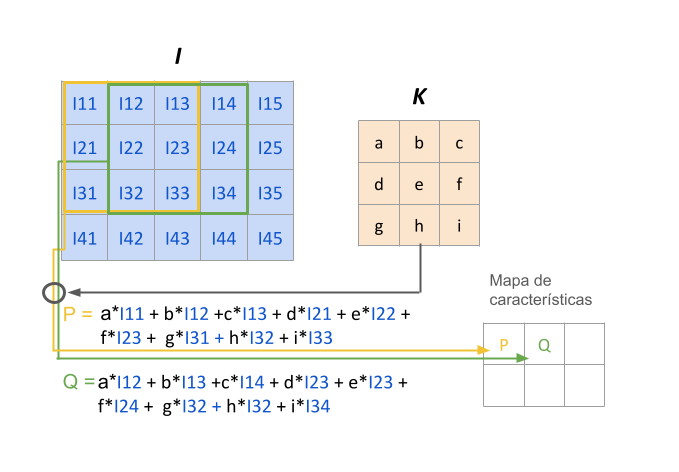
\includegraphics[width=\textwidth]{img/convolucion.png}
         \caption{Convolución reduciendo tamaño.}
         \label{fig:convolucion}
     \end{subfigure}
     \hfill
     \begin{subfigure}[b]{0.45\textwidth}
         \centering
         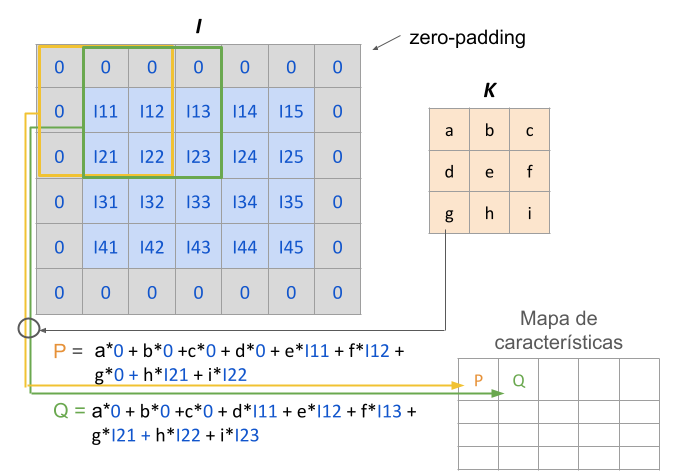
\includegraphics[width=1\textwidth]{img/convolucionPadding.png}
         \caption{Convolución con zero-padding.}
         \label{fig:convolucionPadding}
     \end{subfigure}
     \caption{Convolución en 2D.}
     \label{fig:convolu2}
\end{figure} 

Se observa que el filtro se desplaza por la matriz \textit{I} con paso unitario en vertical y horizontal. Este parámetro se llama stride y su valor depende de el objetivo que se quiera lograr con esta capa convolucional.

\begin{figure}[h]
    \centering
    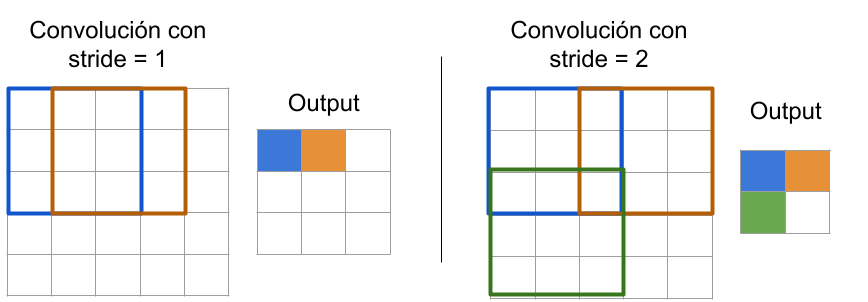
\includegraphics[width=0.6\textwidth]{img/stride.png}
    \caption{Campos receptivos en una convolución. Fuente \citep{yepez2020stride}}
    \label{fig:receptive_field}
\end{figure}

Una longitud de paso de 1 se utiliza normalmente para extraer el máximo número de características, ya que proporciona el máximo solapamiento entre el núcleo y la entrada. Por otro lado, cuando la longitud de paso es mayor que 1, los campos receptivos se solapan menos y producen una salida más pequeña. Si la longitud de paso fuera 3, habría problemas con el espaciado, ya que el campo receptivo no encajaría alrededor de la entrada como un número entero \citep{yepez2020stride}.



Por simplicidad, se ha usado siempre un único kernel, pero se puede generalizar a varios filtros, creando un mapa de características por cada uno. En cada uno de estos mapas hay una neurona por pixel y todas ellas comparten los mismos parámetros, lo que reduce considerablemente el número de parámetros del modelo. El campo receptivo de una neurona ahora se extiende por los mapas de características de todas las capas anteriores \citep{geron2022hands}.



Toda la información anterior se resume en la siguiente ecuación \citep{pajares2021aprendizaje}:

\begin{equation}
z_{i,j,k} = b_k + \sum_{u=0}^{f_h-1} \sum_{v=0}^{f_w-1} \sum_{k'=0}^{f_n'-1} x_{i',j',k'} \cdot w_{u,v,k',k} \hspace{5mm} \textup{con }
\left\{
\begin{array}{l}
i' = i \cdot s_h + u \\
j' = j \cdot s_w + v
\end{array}
\right.
\end{equation}

donde:
\begin{itemize}
    \item \( z_{i,j,k} \) es la salida de la neurona ubicada en la fila \(i\), columna \(j\) en el mapa de características \(k\) de la capa convolucional (capa \(l\)).
    \item \( s_h \) y \( s_w \) son los pasos de avance vertical y horizontal.
    \item \( f_h \) y \( f_w \) son la altura y la anchura del campo receptivo y \( f_{n'} \) es el número de mapas de características de la capa anterior (capa \(l-1\)).
    \item \( x_{i',j',k'} \) es la salida de la neurona situada en la fila \(i'\), columna \(j'\), mapa de características \(k'\).
    \item \( b_k \) es el sesgo para el mapa de características \(k\) (en la capa \(l\)).
    \item \( w_{u,v,k',k} \) es el peso de conexión entre cualquier neurona del mapa de características \(k\) de la capa \(l\) y su entrada situada en la fila \(u\), columna \(v\) (relativa al campo receptivo de la neurona) y el mapa de características \(k'\).
\end{itemize}





\subsubsection*{Capas de pooling}

El siguiente tipo de capa de las \acrshort{cnn} son las pooling, cuyo objetivo es reducir la imagen de entrada para disminuir la carga computacional, el uso de memoria y el número de parámetros, limitando así el riesgo de sobreajuste y proporcionando robustez contra el ruido y las distorsiones. Esta capa se suele colocar entre las capas de convolución, permitiendo reducir el tamaño de las imágenes mientras se preservan las características más importantes \citep{podder2021artificial}. Al igual que en las capas convolucionales, sus neuronas están conectadas a un pequeño grupo de neuronas de la capa anterior a las que se le aplica una función de agregación\footnote{Las funciones de agregación devuelven un valor único de un conjunto de registros.}. Las tres funciones más comunes son el promedio, la suma y el máximo. La Figura \ref{fig:maxpooling} muestra una capa de max pooling, que es el tipo más común \citep{geron2022hands}. 



\begin{figure}[h!]
\centering
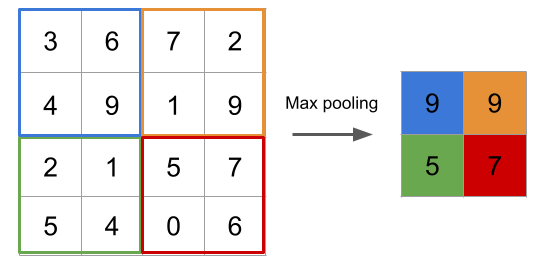
\includegraphics[width=0.4\textwidth]{img/maxpooling.png}
\caption{Capa de max pooling con un kernel de \( 2 \times 2 \), stride 2 y sin padding.}
\label{fig:maxpooling}
\end{figure}

Además de reducir el número de operaciones, el número de parámetros y ayudar con el overfitting, una capa de max pooling introduce cierto nivel de invarianza a pequeñas translaciones, ya que si un pixel se traslada hacia la derecha, la salida también debería trasladarse un pixel hacia la derecha, como se ilustra en la Figura \ref{fig:translacionPooling}. Esto significa que pequeñas variaciones en la posición de las características dentro de la imagen no afectan significativamente la salida.


\begin{figure}[h!]
\centering
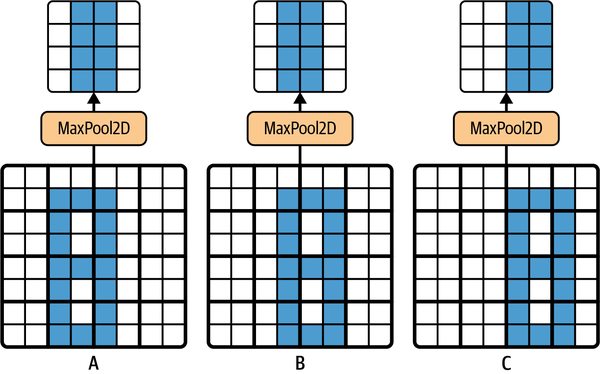
\includegraphics[width=0.4\textwidth]{img/translacionPooling.png}
\caption{Invarianza a translaciones pequeñas mediante una capa de max pooling. Fuente \citep{geron2022hands}}
\label{fig:translacionPooling}
\end{figure}



\subsubsection*{Capas Totalmente Conectadas (Fully Connected)}

Por último están las capas totalmente conectadas (\textit{fully connected}), que realizan la clasificación sobre la salida generada por las capas de convolución y pooling. Como el input de una capa densa debe ser un vector, primero se debe aplanar la salida de la última capa para poder utilizar después esta capa. Cada una de sus neuronas está conectada a todas las de la capa anterior, estableciendo una red densa de conexiones. Este tipo de neuronas suele ir seguido de una capa Dropout para mejorar la generalización del modelo. Este diseño permite a las CNN manejar datos complejos y variados, aprovechando la jerarquía de características aprendidas durante el entrenamiento. Este tipo de capa suele ir seguido de una capa de Dropout que mejora la capacidad de generalización del modelo al prevenir el sobreajuste, un problema común en el ámbito del aprendizaje profundo \citep{hossain2019classification}.



%Adicionalmente, las CNN pueden utilizar técnicas de regularización que ayudan a reducir el sobreajuste. Una de las técnicas más exitosas se llama \textit{dropout} \citep{srivastava2014dropout}. Al entrenar un modelo utilizando \textit{dropout}, durante cada iteración de entrenamiento, un porcentaje especificado de nodos en una capa dada y sus conexiones entrantes y salientes se eliminan aleatoriamente. Incluir \textit{dropout} típicamente mejora la precisión y la capacidad de generalización de un modelo porque aumenta la probabilidad de que un nodo sea útil.

\subsubsection{Aplicaciones y Éxitos}

Los usos de las CNN son significativamente variados. El mayor éxito se ha logrado en tareas de visión por computadora, como la detección y reconocimiento de objetos y escenas \citep{krizhevsky2012imagenet}. Las aplicaciones van desde la biología \citep{ronneberger2015u} hasta el reconocimiento facial \citep{parkhi2015deep}. El mejor ejemplo del éxito de las CNN tuvo lugar en 2012 en la competencia ImageNet, donde una CNN superó el rendimiento de otros métodos y luego la precisión humana en 2015 mediante el uso de GPUs, ReLUs, \textit{dropout} y la generación de imágenes adicionales \citep{he2015delving}. Además, las CNN se han utilizado con éxito en modelos de lenguaje para la detección de fonemas \citep{hinton2012deep}, reconocimiento de letras \citep{lecun1998gradient}, reconocimiento de voz \citep{graves2013speech} y construcción de modelos de lenguaje \citep{collobert2008unified}.



Una de las redes neuronales más importantes y más utilizadas en el campo de la ciberseguridad son la \acrfull{cnn}. Las CNN tienen su origen en el estudio de la corteza visual del cerebro y han sido utilizadas en el reconocimiento de imágenes desde la década de los 80. Actualmente, debido al aumento en la capacidad computacional, la disponibilidad de grandes volúmenes de datos de entrenamiento y las técnicas avanzadas de redes profundas, han permitido que las CNN alcancen un rendimiento excepcional en tareas visuales complejas. Estas redes son la base de servicios como la búsqueda de imágenes o los vehículos autónomos. Además, las CNN no se limitan únicamente a la percepción visual, también han demostrado ser efectivas en tareas como el reconocimiento de voz y el procesamiento del lenguaje natural \citep{geron2022hands}. No obstante, nos enfocaremos únicamente en sus aplicaciones visuales.
\subsection{Red Neuronal Recurrente}
\subsubsection{Restricted Boltzmann Machine}


\section{Bibliotecas utilizadas en Python} \label{Subsec: 3_3}

Para nuestros experimentos, utilizaremos Python debido a su popularidad y versatilidad en el ámbito del aprendizaje automático y la inteligencia artificial. Python ofrece una amplia gama de bibliotecas especializadas que facilitan la creación, entrenamiento y evaluación de modelos, así como el análisis y visualización de datos. A continuación, se describen las principales bibliotecas y frameworks que emplearemos en este trabajo, destacando sus características y ventajas.


\subsection{Principales frameworks. Keras}

Como las técnicas de aprendizaje profundo han ido ganando popularidad, muchas organizaciones académicas e industriales se han centrado en desarrollar marcos para facilitar la experimentación con redes neuronales profundas. En esta sección, ofrecemos una visión general de los marcos de trabajo más importantes que se pueden usar en Python, concluyendo con nuestra elección.


\textbf{TensorFlow} \citep{tensorflow} es una biblioteca de código abierto desarrollada por el equipo de Google Brain para la computación numérica y el aprendizaje automático a gran escala. Diseñada para ser altamente flexible, TensorFlow soporta computación distribuida y permite la optimización de gráficos computacionales, lo que mejora significativamente la velocidad y el uso de memoria de las operaciones. En su núcleo, TensorFlow es similar a NumPy pero con soporte para GPU, lo que acelera considerablemente los cálculos. Además, incluye herramientas avanzadas como TensorBoard para la visualización de modelos y TensorFlow Extended para la producción de modelos de aprendizaje automático. Gracias a estas capacidades, TensorFlow se ha convertido en una herramienta esencial en la industria y la investigación, siendo utilizada en aplicaciones que van desde la clasificación de imágenes y el procesamiento de lenguaje natural hasta los sistemas de recomendación y la previsión de series temporales.


\textbf{Keras} \citep{keras} es una API de alto nivel para redes neuronales que ahora es parte integral de TensorFlow. Fue desarrollada por François Chollet y ganó popularidad rápidamente gracias a su simplicidad y diseño elegante. Inicialmente, Keras soportaba múltiples backends, pero desde la versión 2.4, funciona exclusivamente con TensorFlow \citep{muller2016introduction}. Keras permite a los usuarios construir, entrenar y evaluar modelos de aprendizaje profundo de manera rápida y eficiente. Su facilidad de uso y extensa documentación la convierten en una herramienta valiosa tanto para la investigación como para la implementación de aplicaciones de inteligencia artificial.



\textbf{PyTorch} \citep{pytorch}, desarrollado por el equipo de investigación de IA de Facebook, es una biblioteca de aprendizaje profundo que destaca por su enfoque en la computación dinámica, lo que permite una mayor flexibilidad en la creación de modelos complejos. A diferencia de TensorFlow, que utiliza gráficos computacionales estáticos, PyTorch permite que la topología de la red neuronal cambie durante la ejecución del programa \citep{mahmoud2019dlbench}. Esto, junto con su capacidad de auto-diferenciación en modo inverso\footnote{Técnica en la que PyTorch calcula automáticamente las derivadas de las funciones de pérdida con respecto a los parámetros del modelo.}, hace que PyTorch sea popular entre los investigadores y desarrolladores. Su facilidad de uso y robusta comunidad de apoyo han llevado a su adopción por parte de importantes organizaciones como Facebook, Twitter y NVIDIA.



Para escoger con cuál de estas librerías se realizará la parte práctica de este trabajo, vamos a utilizar, además de las características previamente vistas, los resultados de \citep{mahmoud2019dlbench}. En él se hace un estudio de eficiencia, convergencia, tiempo de entrenamiento y uso de memoria de los diferentes frameworks con varios datasets. Entre sus resultados podemos observar como Keras destaca por encima de las demás en el entorno de la CPU. No solo logra el mejor accuracy en los tres datasets (MNIST, CIFAR-10, CIFAR-100), sino que además también tiene los tiempos de ejecución más bajos y una de las mejores tasas de convergencia. En cuento al entorno de la GPU, las tres librerías obtienen unos resultados semejantes. En conclusión, podemos afirmar que estos resultados junto con su facilidad de uso, accesibilidad y documentación bien estructurada, han sido determinantes para optar por usar Keras en vez de PyTorch o TensorFlow en nuestros estudios posteriores. Aakash Nain resume perfectamente las ventajas de Keras \citep{keraswebsite2} al señalar que:

\begin{quote} 
``Keras is that sweet spot where you get flexibility for research and consistency for deployment. Keras is to Deep Learning what Ubuntu is to Operating Systems.'' 
\end{quote}

De manera similar, Matthew Carrigan destaca la intuitividad y facilidad de uso de Keras \citep{keraswebsite}, afirmando:

\begin{quote}
``The best thing you can say about any software library is that the abstractions it chooses feel completely natural, such that there is zero friction between thinking about what you want to do and thinking about how you want to code it. That's exactly what you get with Keras.''
\end{quote}


\subsection{Librerías y herramientas esenciales.} \label{sec:2.3.2}

De forma complementaria, también es importante conocer y utilizar diversas librerías y herramientas esenciales que facilitan el desarrollo y análisis de los modelos de Keras. Estas incluyen herramientas para la manipulación, visualización y análisis de datos.

\textbf{Scikit-Learn} \citep{scikitlearn} es una librería de código abierto con herramientas simples y eficientes para el análisis predictivo de datos. Contiene varios algoritmos de aprendizaje automático, desde clasificación y regresión hasta clustering y reducción de dimensionalidad, con la documentación completa sobre cada algoritmo. Está construida sobre otras librerías que veremos más adelante como Numpy, SciPy y matplotlib. Aunque no se aprovecharán todas estas funcionalidades de scikit-learn, si que se va a utilizar una de sus funciones más populares, \texttt{train\_test\_split()} \citep{traintestsplit}. Esta función divide el dataset en dos subconjuntos de forma aleatoria, manteniendo la correspondencia en caso de que el dataset contenga dos o más partes. Usualmente, a estos subconjuntos se les llama conjunto de prueba y conjunto de entrenamiento, cuyo tamaño se indica con un valor entre 0 y 1 (\texttt{test\_size}). Además, también se suele asignar una semilla a esa división para que cada vez que se quieran reproducir los experimentos, pueda usarse la misma partición. Esa semilla es un número natural que se introduce como parámetro de entrada en la variable \texttt{random\_state}. Veamos un ejemplo de como utilizar esta función.


\lstset{language=Python}
\begin{lstlisting}
# Ejemplo de codigo en Python
from sklearn.model_selection import train_test_split

X_train, X_test, y_train, y_test = train_test_split(data, labels,
                                        test_size=0.25, random_state=42)
\end{lstlisting}


Las variables X\_train, X\_ test y compañía son numpy arrays. \textbf{NumPy} \citep{numpy} es el paquete fundamental de Python para la computación científica. Es una biblioteca general de estructuras de datos, álgebra lineal y manipulación de matrices para Python, cuya sintaxis y manejo de estructuras de datos y matrices es comparable al de MATLAB \citep{bloice2016tutorial}. En NumPy, se pueden crear arrays y realizar operaciones rápidas y eficientes sobre ellos. Se utilizarán estas estructuras de datos para almacenar los datos y entrenar las redes neuronales con ellas. Aunque también se pueden utilizar tensores \citep{modeltraining}, se ha decidido utilizar numpy arrays por su alta eficiencia operacional y por su uso en la industria.


Otro paquete que se va a utilizar durante los experimentos y que Scikit-Learn utiliza es \textbf{matplotlib} \citep{matplotlib}. Es la principal biblioteca de gráficos científicos en Python y proporciona funciones para crear visualizaciones de calidad como gráficos de barras, histogramas, gráficos de dispersión, etc. Se utilizará este paquete para representar gráficamente los datos de cada dataset para poder obtener bastante información con un simple vistazo. 












\begin{comment}
¿QUITAR?
La ecuación \ref{eq:conv} resume las explicaciones anteriores en una gran ecuación matemática \citep{pajares2021aprendizaje}:

\begin{equation}
z_{i,j,k} = b_k + \sum_{u=0}^{f_h-1} \sum_{v=0}^{f_w-1} \sum_{k'=0}^{f_n'-1} x_{i',j',k'} \cdot w_{u,v,k',k} \hspace{5mm} \textup{con }
\left\{
\begin{array}{l}
i' = i \cdot s_h + u \\
j' = j \cdot s_w + v
\end{array}
\right.
\end{equation} \label{eq:conv}

donde \( z_{i,j,k} \) es la salida de la neurona ubicada en \((i,j)\) en el mapa de características \(k\) de la capa convolucional \(l\). \( s_h \) y \( s_w \) es el stride vertical y horizontal. \( f_h \) y \( f_w \) son las dimensiones del campo receptivo y \( f_{n'} \) es el número de mapas de características de la capa anterior. \( x_{i',j',k'} \) es la salida de la neurona situada en \((i',j')\) y en mapa de características \(k'\). \( b_k \) es el término de sesgo para el mapa de características \(k\) en la capa \(l\) y \( w_{u,v,k',k} \) es el peso de conexión entre cualquier neurona del mapa de características \(k\) de la capa \(l\) y su entrada en \((u,v)\) y el mapa de características \(k'\).
\end{comment}



\begin{comment}
Una de las redes neuronales más importantes y más utilizadas en el campo de la ciberseguridad son las \acrfull{cnn}. Las CNN tienen su origen en el estudio de la corteza visual del cerebro y han sido utilizadas en el reconocimiento de imágenes desde la década de los 80. Actualmente, debido al aumento en la capacidad computacional, la disponibilidad de grandes volúmenes de datos de entrenamiento y las técnicas avanzadas de redes profundas, han permitido que las CNN alcancen un rendimiento excepcional en tareas visuales complejas. Estas redes son la base de servicios como la búsqueda de imágenes o los vehículos autónomos \citep{geron2022hands}.


Una \acrfull{cnn} es una red neuronal diseñada para procesar entradas almacenadas en matrices. Un ejemplo de entrada es una imagen en escala de grises, que es una matriz bidimensional (2D) de píxeles. Aunque estas redes se utilicen principalmente en la clasificación visual de imágenes, también  se han demostrado que son efectivas en tareas como el reconocimiento de voz (matrices 2D de imágenes o espectrogramas de audio) \citep{kim2023bilstm}, clasificación visual de videos o imágenes volumétricas (matrices tridimensionales 3D) \citep{diba2017temporal} y procesamiento de lenguaje natural(matriz 2D) \citep{wang2017combining}. Independientemente de la dimensionalidad, las CNN se utilizan donde hay un ordenamiento espacial o temporal \citep{berman2019survey}. No obstante, nos enfocaremos únicamente en sus aplicaciones visuales.

La arquitectura de una CNN (ver Figura ????????) consta de tres tipos distintos de capas: capas de convolución, capas de pooling y la capa de clasificación. 

IMAGEN CAPAS: \citep{phung2018deep}


\subsubsection*{Capas convolucionales}

La capa convolucional es el bloque de construcción más importante de una red neuronal convolucional (CNN). En ella se aplica la operación de convolución, que involucra dos funciones y produce una tercera función que representa la cantidad de superposición de una función a medida que se desplaza sobre otra. Supóngase que se tiene una fuente de luz variable cuya intensidad se recibe mediante un sensor. Este sensor proporciona una salida en una determinada posición \( x \) en el tiempo \( t \), esto es, \( x(t) \). Tanto \( x \) como \( t \) son valores reales, de forma que debido a la variabilidad de la fuente mencionada, se pueden obtener diferentes lecturas en diferentes instantes de tiempo. La captura de la señal por el sensor puede estar contaminada con cierto ruido. Para obtener una señal más limpia, lo acertado es realizar un promediado de la salida con varias medidas. Si además tenemos en cuenta que las medidas más recientes son más relevantes que las alejadas en el tiempo, el promediado puede ponderarse concediendo más relevancia a las medidas recientes. Esto puede hacerse mediante una función de promediado \( w(a) \), donde \( a \) representa el alejamiento de la medida en el tiempo. Si se realiza esta operación de promediado ponderado en cada instante de tiempo \( t \), se obtiene una nueva función promediada como sigue:

\begin{equation}
s(t) = \int x(a) w(t-a) \, da
\end{equation}

Esta operación se denomina convolución, y se denota como:

\begin{equation}
s(t) = \int (x \star w)(t)
\end{equation}

Para que el promedio ponderado sea válido, la función de promediado \( w(t) \) necesita ser una función de densidad de probabilidad. Además, \( w(t) \) debe ser cero para todos los valores negativos de \( t \) para evitar tomar valores futuros, lo cual no es físicamente posible \citep{pajares2021aprendizaje}.


Para aplicaciones prácticas como el procesamiento de imágenes, las medidas suelen ser discretas, es decir, se toman en intervalos de tiempo específicos. En este caso, el tiempo \( t \) toma valores enteros, y la convolución discreta se define como:

\begin{equation}
s(t) = (x \star w)(t) = \sum_{a=-\infty}^{\infty} x(a) w(t-a)
\end{equation}

En el contexto de las CNN, la entrada es un vector o matriz multidimensional de datos (la imagen), y el núcleo es una matriz multidimensional de parámetros que se ajustan durante el proceso de aprendizaje. Sea \( I \) la imagen de entrada y \( K \) un núcleo de convolución. Se define la convolución discreta en dos dimensiones como:

\begin{equation}
S(i, j) = (K \star I)(i, j) = \sum_{m=0}^{M-1} \sum_{n=0}^{N-1} I(i+m, j+n) K(m, n)
\end{equation}

donde \( M \) y \( N \) son las dimensiones del núcleo. La figura ????? muestra un ejemplo de convolución con el núcleo \( K \), aplicado sobre una imagen \( I \). 


En una CNN, esta construcción es la mas importante. Las neuronas de la primera capa convolucional se concectan a todos y cada uno de los píxeles de la imagen de entrada, sino solo a píxeles en sus campos receptivos. A su vez, cada neurona de la segunda capa convolucional está conectada a las neuronas ubicadas dentro de un rectángulo pequeño en la primera capa. Esta arquitectura permite a la red concentrarse en cracterísticas pequeñas de bajo nivel en la primera capa oculta, juntarlas después para crear características más grandes de nivel superior en la siguiente capa oculta, y así sucesivamente. La convolución se realiza con solapamiento total del núcleo, lo que resulta en una imagen resultante de menor dimensión (REFERENCIA IMAGEN A ?????). Si se desea mantener la misma dimensión, se puede aplicar relleno con ceros o zero-padding (REFERENCIA IMAGEN A ?????). Este relleno se indica como "same" en términos de implementación. Si no se realiza relleno con ceros, se indica como "valid". Por otra parte, en las convoluciones, el campo receptivo se define como la región de entrada que contribuye a la salida generada por el filtro. En la figura REFERENCIA IMAGEN A ?????) se muestran sendos campos receptivos de la imagen \( I \) que contribuyen a las salidas \( P \) y \( \Q \) generadas por el filtro \( K \).


IMAGENES PADDING

Por último, se define el stride. Stride es la longitud de paso de desplazamiento del núcleo alrededor de la entrada. Cuando la longitud de paso es 1, el núcleo se desplaza sobre la entrada un elemento a la vez. Normalmente, la longitud de paso se establece de manera que el volumen de salida sea un número entero.

FOTOOO stride Fuente:\citep{yepez2020stride}

La Figura de la izquierda muestra una entrada de \(5 \times 5\) con un núcleo de \(3 \times 3\). Con un stride de paso 1, se genera una matriz de salida de tamaño \(3 \times 3\). Una longitud de paso de 1 se utiliza normalmente para extraer el máximo número de características, ya que proporciona el máximo solapamiento entre el núcleo y la entrada, pero a máxima complejidad computacional. Por otro lado, la imagen de la derecha muestra el núcleo desplazándose dos unidades sobre la entrada, generando una matriz de salida de \(2 \times 2\). Generalmente, cuando la longitud de paso es mayor que 1, los campos receptivos se solapan menos y producen una salida más pequeña. Si la longitud de paso fuera 3, habría problemas con el espaciado, ya que el campo receptivo no encajaría alrededor de la entrada como un número entero \citep{yepez2020stride}.









cada neurona en la capa convolucional está conectada solo a una pequeña región de la imagen de entrada (campo receptivo). Estas conexiones se realizan utilizando filtros (o núcleos de convolución), y la salida se conoce como mapa de características. La ecuación \ref{eq:conv} resume las explicaciones anteriores en una gran ecuación matemática \citep{pajares2021aprendizaje}:

\begin{equation}
z_{i,j,k} = b_k + \sum_{u=0}^{f_h-1} \sum_{v=0}^{f_w-1} \sum_{k'=0}^{f_n'-1} x_{i',j',k'} \cdot w_{u,v,k',k} \hspace{5mm} \textup{con }
\left\{
\begin{array}{l}
i' = i \cdot s_h + u \\
j' = j \cdot s_w + v
\end{array}
\right.
\end{equation}

donde:
\begin{itemize}
    \item \( z_{i,j,k} \) es la salida de la neurona ubicada en la fila \(i\), columna \(j\) en el mapa de características \(k\) de la capa convolucional (capa \(l\)).
    \item \( s_h \) y \( s_w \) son los pasos de avance vertical y horizontal.
    \item \( f_h \) y \( f_w \) son la altura y la anchura del campo receptivo y \( f_{n'} \) es el número de mapas de características de la capa anterior (capa \(l-1\)).
    \item \( x_{i',j',k'} \) es la salida de la neurona situada en la fila \(i'\), columna \(j'\), mapa de características \(k'\) (o canal \(k'\) si la capa anterior es la capa de entrada).
    \item \( b_k \) es el término de sesgo para el mapa de características \(k\) (en la capa \(l\)). Puedes imaginarlo como una rueda que ajusta el brillo general del mapa de características \(k\).
    \item \( w_{u,v,k',k} \) es el peso de conexión entre cualquier neurona del mapa de características \(k\) de la capa \(l\) y su entrada situada en la fila \(u\), columna \(v\) (relativa al campo receptivo de la neurona) y el mapa de características \(k'\).
\end{itemize}









\subsection{Red Neuronal Convolucional}

Una de las redes neuronales más importantes y más utilizadas en el campo de la ciberseguridad son las \acrfull{cnn}. Las CNN tienen su origen en el estudio de la corteza visual del cerebro y han sido utilizadas en el reconocimiento de imágenes desde la década de los 80. Actualmente, debido al aumento en la capacidad computacional, la disponibilidad de grandes volúmenes de datos de entrenamiento y las técnicas avanzadas de redes profundas, han permitido que las CNN alcancen un rendimiento excepcional en tareas visuales complejas. Estas redes son la base de servicios como la búsqueda de imágenes o los vehículos autónomos \citep{geron2022hands}.

Una \acrfull{cnn} es una red neuronal diseñada para procesar entradas almacenadas en matrices. Un ejemplo de entrada es una imagen en escala de grises, que es una matriz bidimensional (2D) de píxeles. Aunque estas redes se utilicen principalmente en la clasificación visual de imágenes, también se ha demostrado que son efectivas en tareas como el reconocimiento de voz (matrices 2D de imágenes o espectrogramas de audio) \citep{kim2023bilstm}, clasificación visual de videos o imágenes volumétricas (matrices tridimensionales 3D) \citep{diba2017temporal} y procesamiento de lenguaje natural (matriz 2D) \citep{wang2017combining}. Independientemente de la dimensionalidad, las CNN se utilizan donde hay un ordenamiento espacial o temporal \citep{berman2019survey}. No obstante, nos enfocaremos únicamente en sus aplicaciones visuales.

La arquitectura de una CNN (ver Figura ????????) consta de tres tipos distintos de capas: capas de convolución, capas de pooling y la capa de clasificación.

\begin{figure}[h]
    \centering
    \includegraphics[width=0.8\textwidth]{path_to_image}
    \caption{Arquitectura de una CNN con capas de convolución, pooling y clasificación \citep{phung2018deep}.}
    \label{fig:cnn_architecture}
\end{figure}

\subsubsection*{Capas convolucionales}

La capa convolucional es el bloque de construcción más importante de una \fullacr{cnn}. En ella se aplica la operación de convolución, que involucra dos funciones y produce una tercera función que representa la cantidad de superposición de una función a medida que se desplaza sobre otra. Supóngase que se tiene una fuente de luz variable cuya intensidad se recibe mediante un sensor. Este sensor proporciona una salida en una determinada posición \( x \) en el tiempo \( t \), esto es, \( x(t) \). Tanto \( x \) como \( t \) son valores reales, de forma que debido a la variabilidad de la fuente mencionada, se pueden obtener diferentes lecturas en diferentes instantes de tiempo. La captura de la señal por el sensor puede estar contaminada con cierto ruido. Para obtener una señal más limpia, lo acertado es realizar un promediado de la salida con varias medidas. Si además tenemos en cuenta que las medidas más recientes son más relevantes que las alejadas en el tiempo, el promediado puede ponderarse concediendo más relevancia a las medidas recientes. Esto puede hacerse mediante una función de promediado \( w(a) \), donde \( a \) representa el alejamiento de la medida en el tiempo. Si se realiza esta operación de promediado ponderado en cada instante de tiempo \( t \), se obtiene una nueva función promediada como sigue:

\begin{equation}
s(t) = \int x(a) w(t-a) \, da
\end{equation}

Esta operación se denomina convolución, y se denota como:

\begin{equation}
s(t) = \int (x \star w)(t)
\end{equation}

Para que el promedio ponderado sea válido, la función de promediado \( w(t) \) necesita ser una función de densidad de probabilidad. Además, \( w(t) \) debe ser cero para todos los valores negativos de \( t \) para evitar tomar valores futuros, lo cual no es físicamente posible \citep{pajares2021aprendizaje}.


Para aplicaciones prácticas como el procesamiento de imágenes, las medidas suelen ser discretas, es decir, se toman en intervalos de tiempo específicos. En este caso, el tiempo \( t \) toma valores enteros, y la convolución discreta se define como:

\begin{equation}
s(t) = (x \star w)(t) = \sum_{a=-\infty}^{\infty} x(a) w(t-a)
\end{equation}

En el contexto de las CNN, la entrada es un vector o matriz multidimensional de datos (la imagen), y el núcleo es una matriz multidimensional de parámetros que se ajustan durante el proceso de aprendizaje. Sea \( I \) la imagen de entrada y \( K \) un núcleo de convolución. Se define la convolución discreta en dos dimensiones como:

\begin{equation}
S(i, j) = (K \star I)(i, j) = \sum_{m=0}^{M-1} \sum_{n=0}^{N-1} I(i+m, j+n) K(m, n)
\end{equation}

donde \( M \) y \( N \) son las dimensiones del núcleo. La figura \ref{fig:conv_example} muestra un ejemplo de convolución con el núcleo \( K \), aplicado sobre una imagen \( I \).

\begin{figure}[h]
    \centering
    \includegraphics[width=0.8\textwidth]{path_to_image}
    \caption{Ejemplo de convolución con un núcleo \( K \) aplicado sobre una imagen \( I \).}
    \label{fig:conv_example}
\end{figure}

En una CNN, esta construcción es la más importante. Las neuronas de la primera capa convolucional no se conectan a todos y cada uno de los píxeles de la imagen de entrada, sino solo a píxeles en sus campos receptivos. A su vez, cada neurona de la segunda capa convolucional está conectada a las neuronas ubicadas dentro de un rectángulo pequeño en la primera capa. Esta arquitectura permite a la red concentrarse en características pequeñas de bajo nivel en la primera capa oculta, juntarlas después para crear características más grandes de nivel superior en la siguiente capa oculta, y así sucesivamente. La convolución se realiza con solapamiento total del núcleo, lo que resulta en una imagen resultante de menor dimensión (ver Figura \ref{fig:padding_valid}). Si se desea mantener la misma dimensión, se puede aplicar relleno con ceros o zero-padding (ver Figura \ref{fig:padding_same}). Este relleno se indica como "same" en términos de implementación. Si no se realiza relleno con ceros, se indica como "valid". Por otra parte, en las convoluciones, el campo receptivo se define como la región de entrada que contribuye a la salida generada por el filtro. En la figura \ref{fig:receptive_field} se muestran sendos campos receptivos de la imagen \( I \) que contribuyen a las salidas \( P \) y \( Q \) generadas por el filtro \( K \).

\begin{figure}[h]
    \centering
    \includegraphics[width=0.8\textwidth]{path_to_image}
    \caption{Convolución con relleno "valid".}
    \label{fig:padding_valid}
\end{figure}

\begin{figure}[h]
    \centering
    \includegraphics[width=0.8\textwidth]{path_to_image}
    \caption{Convolución con relleno "same".}
    \label{fig:padding_same}
\end{figure}

\begin{figure}[h]
    \centering
    \includegraphics[width=0.8\textwidth]{path_to_image}
    \caption{Campos receptivos en una convolución.}
    \label{fig:receptive_field}
\end{figure}

Por último, se define el stride. Stride es la longitud de paso de desplazamiento del núcleo alrededor de la entrada. Cuando la longitud de paso es 1, el núcleo se desplaza sobre la entrada un elemento a la vez. Normalmente, la longitud de paso se establece de manera que el volumen de salida sea un número entero.

\begin{figure}[h]
    \centering
    \includegraphics[width=0.8\textwidth]{path_to_image}
    \caption{Ejemplo de convolución con diferentes strides. Fuente: \citep{yepez2020stride}.}
    \label{fig:stride_example}
\end{figure}

La Figura \ref{fig:stride_example} de la izquierda muestra una entrada de \(5 \times 5\) con un núcleo de \(3 \times 3\). Con un stride de paso 1, se genera una matriz de salida de tamaño \(3 \times 3\). Una longitud de paso de 1 se utiliza normalmente para extraer el máximo número de características, ya que proporciona el máximo solapamiento entre el núcleo y la entrada, pero a máxima complejidad computacional. Por otro lado, la imagen de la derecha muestra el núcleo desplazándose dos unidades sobre la entrada, generando una matriz de salida de \(2 \times 2\). Generalmente, cuando la longitud de paso es mayor que 1, los campos receptivos se solapan menos y producen una salida más pequeña. Si la longitud de paso fuera 3, habría problemas con el espaciado, ya que el campo receptivo no encajaría alrededor de la entrada como un número entero.



La ecuación \ref{eq:conv} resume las explicaciones anteriores en una gran ecuación matemática \citep{pajares2021aprendizaje}:

\begin{equation}
z_{i,j,k} = b_k + \sum_{u=0}^{f_h-1} \sum_{v=0}^{f_w-1} \sum_{k'=0}^{f_n'-1} x_{i',j',k'} \cdot w_{u,v,k',k} \hspace{5mm} \textup{con }
\left\{
\begin{array}{l}
i' = i \cdot s_h + u \\
j' = j \cdot s_w + v
\end{array}
\right.
\end{equation}

donde:
\begin{itemize}
    \item \( z_{i,j,k} \) es la salida de la neurona ubicada en la fila \(i\), columna \(j\) en el mapa de características \(k\) de la capa convolucional (capa \(l\)).
    \item \( s_h \) y \( s_w \) son los pasos de avance vertical y horizontal.
    \item \( f_h \) y \( f_w \) son la altura y la anchura del campo receptivo y \( f_{n'} \) es el número de mapas de características de la capa anterior (capa \(l-1\)).
    \item \( x_{i',j',k'} \) es la salida de la neurona situada en la fila \(i'\), columna \(j'\), mapa de características \(k'\) (o canal \(k'\) si la capa anterior es la capa de entrada).
    \item \( b_k \) es el término de sesgo para el mapa de características \(k\) (en la capa \(l\)).
    \item \( w_{u,v,k',k} \) es el peso de conexión entre cualquier neurona del mapa de características \(k\) de la capa \(l\) y su entrada situada en la fila \(u\), columna \(v\) (relativa al campo receptivo de la neurona) y el mapa de características \(k'\).
\end{itemize}
\end{comment}




\begin{comment}

\textbf{MXNet} \citep{mxnet} es un marco de trabajo de aprendizaje profundo de código abierto fundado como una colaboración entre la Universidad Carnegie Mellon, la Universidad de Washington y Microsoft. Es una librería escalable que permite el entrenamiento de redes neuronales profundas utilizando diferentes lenguajes de programación, incluyendo C++, Python, MATLAB, JavaScript, R, Julia y Scala. MXNet incluye la interfaz de Gluon que permite a los desarrolladores con cualquier nivel de experiencia comenzar a usar el aprendizaje profundo en la nube, en dispositivos de borde \footnote{dispositivos más cercanos al usuario, como teléfonos móviles, sistemas ciberfísicos (CPS), dispositivos portátiles, IoT, \ldots.} y en aplicaciones para dispositivos móviles. MXNet admite además el paralelismo de datos en múltiples CPUs o GPUs, así como el paralelismo de modelos. Ofrece dos modos de entrenamiento diferentes: síncrono y asíncrono \footnote{síncrono: interactúan en el mismo momento en el que tiene lugar la comunicación; asíncrono: la interacción no es inmediata y puede tener lugar en momentos diferentes} y además proporciona operaciones primitivas de tolerancia a fallas a través de guardar y cargar: guardar almacena los parámetros del modelo en un archivo de punto de control y cargar restaura los parámetros del modelo desde un archivo de punto de control. MXNet admite tanto la programación declarativa como la programación imperativa.
\textbf{Theano} \citep{theano} es una biblioteca de Python de código abierto para cálculos a gran escala que ha sido desarrollado por investigadores y desarrolladores de la Universidad de Montreal. Es una biblioteca que facilita la construcción de modelos de aprendizaje profundo y se puede ejecutar en diferentes plataformas informáticas, incluyendo CPU y GPU. Los cálculos se expresan utilizando una sintaxis similar a la de Numpy y funciona creando una representación simbólica de las operaciones que se traducen a C++ y luego se compilan en moléculas Python. Theano admite tanto el paralelismo de datos como el paralelismo de modelos.
\textbf{Chainer} \citep{chainer} es un marco de aprendizaje profundo de código abierto implementado en Python. El desarrollo de Chainer está liderado por investigadores y desarrolladores de la Universidad de Tokio. Chainer proporciona APIs de diferenciación automática para construir y entrenar redes neuronales, con un enfoque de ``definir por ejecutar'', lo que permite construir el grafo computacional durante el entrenamiento y permite al usuario cambiarlo en cada iteración. Chainer es un marco flexible ya que proporciona una API imperativa en Python y NumPy. Se admiten tanto cálculos en CPU como en GPU.
\end{comment}









